\chapter{Opis problemu}

W większości przypadków aplikacje z przeznaczeniem dla systemu Android pisane są według następującego schematu:

\begin{figure}[!htb]
    \centering
    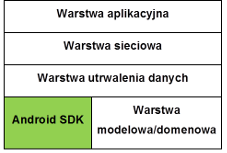
\includegraphics[width=15cm]{imgs/ch3_opis_problemu_1.png}
    \caption
{Podejście „standardowe” przy tworzeniu aplikacji dla systemu Android}
    \label{fig:opis_problemu}
\end{figure} 

Czyli, na najniższej warstwie mamy Android SDK (Software Development Kit) i na niej budujemy kolejne warstwy. Każda z kolejnych warstw naszego oprogramowania korzysta z warstwy poniżej, a co za tym idzie, dziedziczy również zależności z warstwy Android SDK. Analizując taką strukturę aplikacji dostępnych pod Androidem możemy zaobserwować, że w wielu z nich:
\begin{itemize}
\item
nie jest zachowana zasada pojedynczej odpowiedzialności,
\item
warstwa odpowiedzialna za logikę domenową jest pomieszana z warstwą UI (User Interface),
\item
logika UI jest pomieszana z asynchronicznym pobieraniem danych,
\item
funkcje callback możemy znaleźć dosłownie wszędzie,
\item
elementy warstwy UI: Activity i Fragmenty potrafią mieć tysiące linii kodu,
\item
w większości plików aplikacji na każdej warstwie odwołujemy się do środowiska Android (import android.*)
\item
i ostatnie, ale najważniejsze z punktu widzenia tej pracy: jeżeli w kodzie źródłowym szukamy zestawu unit testów – możemy się rozczarować.
\end{itemize}

Spowodowane jest to dwoma czynnikami: pierwszy to trudność w wyodrębnieniu obszarów testowych z powodu zbyt dużego sprzężenia między warstwami (wspomnianego już \textit{couplingu}), a drugi – pracochłonność w pisaniu testów. Jeżeli granica pomiędzy kolejnymi warstwami oprogramowania nie jest jasno wyznaczona, liczba testów do zaprojektowania rośnie drastycznie. Wyjaśnię to na poniższym przykładzie:

Weźmy dwie funkcjonalności: funkcjonalność \textbf{A} opisaną za pomocą kodu z jedną instrukcją warunkową \textit{„if”}, oraz funkcjonalność \textbf{B}, w której mamy dwie zależne od siebie instrukcje \textit{„if”}, czyli cztery możliwe decyzje programowe. Testując te funkcjonalności razem (z powodu sprzężenia nie mamy innego wyjścia) musimy wykonać łącznie \textit{2 * 4 = 8} testów. Testy te równocześnie przestają być unit testami, gdyż łączą w sobie kilka funkcjonalności i stają się przez to testami integracyjnymi. Testując natomiast te funkcjonalności osobno, wykonamy \textit{2 + 4 = 6} unit testów. W tym przykładzie oczywiście nie widać zbyt wielkiej optymalizacji, ale w aplikacjach z kodem, który dostarcza setki czy tysiące decyzji, różnica będzie znacząca.

\colorbox{red}{(dodać rysunki i ilustracje przedstawiające szerzej przykład)}

\newpage
Z doświadczenia własnego oraz kolegów testerów wiem, że jeżeli chcemy aplikację przetestować zaczynając od testów integracyjnych zamiast od unit testu, nakład pracy będzie zdecydowanie większy, niż gdy zastosujemy schemat standardowy, czyli zaczynając od unit testów, kontynuując poprzez testy integracyjne, następnie systemowe, a kończąc na akceptacyjnych (etapów może być więcej). Pozbawiając się możliwości zastosowania unit testów we wczesnym etapie projektu z powodu źle zaprojektowanej struktury aplikacji, ryzykujemy utratę jakości, a co za tym idzie - utratę zaufania klientów do naszego oprogramowania. Idealna piramida testowania, spopularyzowana przez Mike’a Cohna \footnote{Mike Cohn jest jednym twórców metodologii tworzenia oprogramowania Scrum. Jest jednym z założycieli Scrum Alliance oraz właścicielem Mountain Goat Software, firmy, która oferuje szkolenia na Scrum i technik Agile.}  w książce „Succeeding with Agile” \cite{bib:cohn:agile}, przedstawiona została na rysunku \ref{fig:idealna_piramida}.

\begin{figure}[!htb]
    \centering
    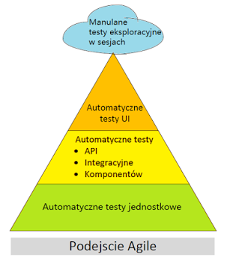
\includegraphics[width=10cm]{imgs/ch3_idealna_piramida.png}
    \caption
{Idealna piramida testowania według Mike'a Cohna\cite{bib:cohn:agile}}
    \label{fig:idealna_piramida}
\end{figure} 

Z powyższego schematu wynika, że idealnie byłoby, gdyby wszystkie etapy testów zostały zautomatyzowane (wszystkie, z wyjątkiem manualnych testów akceptacyjnych, ale w idealnym świecie powinno być ich tak mało, że ich automatyzacja nie miałaby większego sensu). Oczywiście piramida ta może przybierać różne formy, poziomów testowania może być więcej lub mniej, mogą być one zautomatyzowane lub nie, ale idea jest cały czas ta sama: najwięcej testów powinno być na najniższym poziomie. Powinny być one również najprostsze do zaprojektowania. Im dalsza faza projektu, tym testy stają się bardziej pracochłonne, a koszt usunięcia znalezionego błędu wyższy, do czego autor nawiązał już w tabeli \ref{tab:koszty_bledu}.

Wracając do analizy oprogramowania na platformę Android, aktualnie w większości przypadków schemat ten wygląda jednak tak jak na rysunku \ref{fig:odwrocona_piramida}.

\begin{figure}[!htb]
    \centering
    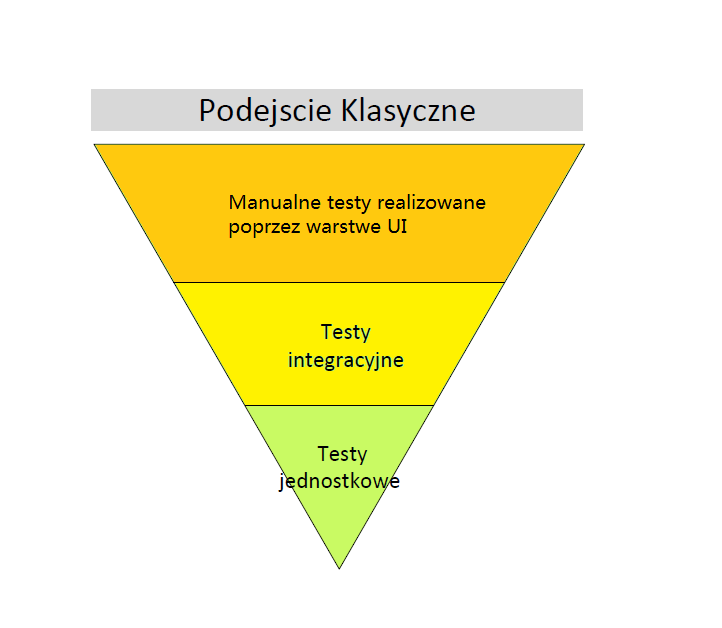
\includegraphics[width=8cm]{imgs/ch3_odwrocona_piramida.png}
    \caption
{Software Testing Ice Cream AntiPatern. Źródło: watirmelon.com}
    \label{fig:odwrocona_piramida}
\end{figure} 

Na rysunku \ref{fig:odwrocona_piramida} widać, że z powodu zbyt dużego \textit{couplingu} unit testy zastąpione zostają testami integracyjnymi, a najwięcej przypadków testowych wykonywanych jest na interfejsie użytkownika (w czym znacznie pomagają frameworki testowe pozwalające na zautomatyzowanie pewnych czynności, nagranie makr według specyfikacji lub \textit{„user stories”}) oraz testy manualne.

Autor nie zaprzecza, że tym sposobem nie da się dobrze przetestować aplikacji, szczególnie że według podręczników testerskich testowanie gruntowne nie jest możliwe, jakiejkolwiek metody nie użylibyśmy. Lecz ryzyko znalezienia błędu na dalszym etapie projektu jest w tym przypadku znacznie większe niż w przypadku oprogramowania o usystematyzowanej strukturze, a co za tym idzie – koszty jego usunięcia są również znacznie wyższe.

Propozycję rozwiązania problemu autor przybliży w kolejnym rozdziale.